% Created by tikzDevice version 0.12 on 2019-04-30 13:35:46
% !TEX encoding = UTF-8 Unicode
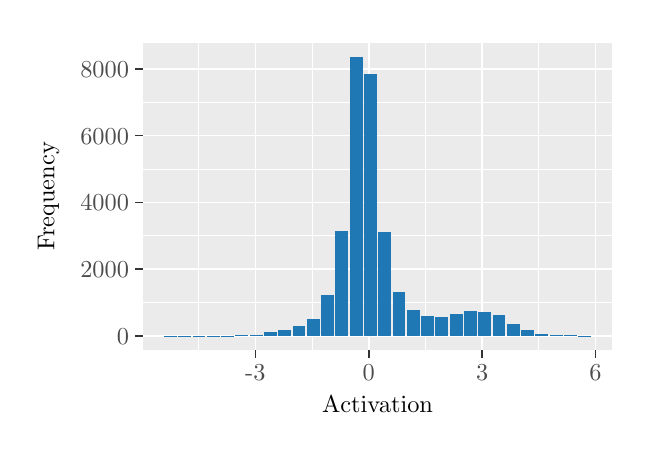
\begin{tikzpicture}[x=1pt,y=1pt]
\definecolor{fillColor}{RGB}{255,255,255}
\path[use as bounding box,fill=fillColor,fill opacity=0.00] (0,0) rectangle (216.81,144.54);
\begin{scope}
\path[clip] (  0.00,  0.00) rectangle (216.81,144.54);
\definecolor{drawColor}{RGB}{255,255,255}
\definecolor{fillColor}{RGB}{255,255,255}

\path[draw=drawColor,line width= 0.6pt,line join=round,line cap=round,fill=fillColor] (  0.00,  0.00) rectangle (216.81,144.54);
\end{scope}
\begin{scope}
\path[clip] ( 41.55, 28.07) rectangle (211.31,139.04);
\definecolor{fillColor}{gray}{0.92}

\path[fill=fillColor] ( 41.55, 28.07) rectangle (211.31,139.04);
\definecolor{drawColor}{RGB}{255,255,255}

\path[draw=drawColor,line width= 0.3pt,line join=round] ( 41.55, 45.18) --
	(211.31, 45.18);

\path[draw=drawColor,line width= 0.3pt,line join=round] ( 41.55, 69.32) --
	(211.31, 69.32);

\path[draw=drawColor,line width= 0.3pt,line join=round] ( 41.55, 93.46) --
	(211.31, 93.46);

\path[draw=drawColor,line width= 0.3pt,line join=round] ( 41.55,117.59) --
	(211.31,117.59);

\path[draw=drawColor,line width= 0.3pt,line join=round] ( 61.79, 28.07) --
	( 61.79,139.04);

\path[draw=drawColor,line width= 0.3pt,line join=round] (102.76, 28.07) --
	(102.76,139.04);

\path[draw=drawColor,line width= 0.3pt,line join=round] (143.73, 28.07) --
	(143.73,139.04);

\path[draw=drawColor,line width= 0.3pt,line join=round] (184.70, 28.07) --
	(184.70,139.04);

\path[draw=drawColor,line width= 0.6pt,line join=round] ( 41.55, 33.12) --
	(211.31, 33.12);

\path[draw=drawColor,line width= 0.6pt,line join=round] ( 41.55, 57.25) --
	(211.31, 57.25);

\path[draw=drawColor,line width= 0.6pt,line join=round] ( 41.55, 81.39) --
	(211.31, 81.39);

\path[draw=drawColor,line width= 0.6pt,line join=round] ( 41.55,105.53) --
	(211.31,105.53);

\path[draw=drawColor,line width= 0.6pt,line join=round] ( 41.55,129.66) --
	(211.31,129.66);

\path[draw=drawColor,line width= 0.6pt,line join=round] ( 82.28, 28.07) --
	( 82.28,139.04);

\path[draw=drawColor,line width= 0.6pt,line join=round] (123.25, 28.07) --
	(123.25,139.04);

\path[draw=drawColor,line width= 0.6pt,line join=round] (164.22, 28.07) --
	(164.22,139.04);

\path[draw=drawColor,line width= 0.6pt,line join=round] (205.19, 28.07) --
	(205.19,139.04);
\definecolor{fillColor}{RGB}{31,120,180}

\path[fill=fillColor] ( 49.27, 33.12) rectangle ( 53.91, 33.13);

\path[fill=fillColor] ( 54.43, 33.12) rectangle ( 59.07, 33.14);

\path[fill=fillColor] ( 59.59, 33.12) rectangle ( 64.24, 33.15);

\path[fill=fillColor] ( 64.75, 33.12) rectangle ( 69.40, 33.19);

\path[fill=fillColor] ( 69.91, 33.12) rectangle ( 74.56, 33.25);

\path[fill=fillColor] ( 75.07, 33.12) rectangle ( 79.72, 33.43);

\path[fill=fillColor] ( 80.24, 33.12) rectangle ( 84.88, 33.63);

\path[fill=fillColor] ( 85.40, 33.12) rectangle ( 90.04, 34.46);

\path[fill=fillColor] ( 90.56, 33.12) rectangle ( 95.20, 35.19);

\path[fill=fillColor] ( 95.72, 33.12) rectangle (100.37, 36.63);

\path[fill=fillColor] (100.88, 33.12) rectangle (105.53, 39.22);

\path[fill=fillColor] (106.04, 33.12) rectangle (110.69, 48.02);

\path[fill=fillColor] (111.20, 33.12) rectangle (115.85, 71.00);

\path[fill=fillColor] (116.37, 33.12) rectangle (121.01,134.00);

\path[fill=fillColor] (121.53, 33.12) rectangle (126.17,127.62);

\path[fill=fillColor] (126.69, 33.12) rectangle (131.33, 70.77);

\path[fill=fillColor] (131.85, 33.12) rectangle (136.50, 49.07);

\path[fill=fillColor] (137.01, 33.12) rectangle (141.66, 42.44);

\path[fill=fillColor] (142.17, 33.12) rectangle (146.82, 40.38);

\path[fill=fillColor] (147.33, 33.12) rectangle (151.98, 40.12);

\path[fill=fillColor] (152.50, 33.12) rectangle (157.14, 41.04);

\path[fill=fillColor] (157.66, 33.12) rectangle (162.30, 42.11);

\path[fill=fillColor] (162.82, 33.12) rectangle (167.46, 41.88);

\path[fill=fillColor] (167.98, 33.12) rectangle (172.63, 40.60);

\path[fill=fillColor] (173.14, 33.12) rectangle (177.79, 37.58);

\path[fill=fillColor] (178.30, 33.12) rectangle (182.95, 35.24);

\path[fill=fillColor] (183.46, 33.12) rectangle (188.11, 33.95);

\path[fill=fillColor] (188.63, 33.12) rectangle (193.27, 33.55);

\path[fill=fillColor] (193.79, 33.12) rectangle (198.43, 33.33);

\path[fill=fillColor] (198.95, 33.12) rectangle (203.59, 33.14);
\end{scope}
\begin{scope}
\path[clip] (  0.00,  0.00) rectangle (216.81,144.54);
\definecolor{drawColor}{gray}{0.30}

\node[text=drawColor,anchor=base east,inner sep=0pt, outer sep=0pt, scale=  0.88] at ( 36.60, 30.09) {0};

\node[text=drawColor,anchor=base east,inner sep=0pt, outer sep=0pt, scale=  0.88] at ( 36.60, 54.22) {2000};

\node[text=drawColor,anchor=base east,inner sep=0pt, outer sep=0pt, scale=  0.88] at ( 36.60, 78.36) {4000};

\node[text=drawColor,anchor=base east,inner sep=0pt, outer sep=0pt, scale=  0.88] at ( 36.60,102.50) {6000};

\node[text=drawColor,anchor=base east,inner sep=0pt, outer sep=0pt, scale=  0.88] at ( 36.60,126.63) {8000};
\end{scope}
\begin{scope}
\path[clip] (  0.00,  0.00) rectangle (216.81,144.54);
\definecolor{drawColor}{gray}{0.20}

\path[draw=drawColor,line width= 0.6pt,line join=round] ( 38.80, 33.12) --
	( 41.55, 33.12);

\path[draw=drawColor,line width= 0.6pt,line join=round] ( 38.80, 57.25) --
	( 41.55, 57.25);

\path[draw=drawColor,line width= 0.6pt,line join=round] ( 38.80, 81.39) --
	( 41.55, 81.39);

\path[draw=drawColor,line width= 0.6pt,line join=round] ( 38.80,105.53) --
	( 41.55,105.53);

\path[draw=drawColor,line width= 0.6pt,line join=round] ( 38.80,129.66) --
	( 41.55,129.66);
\end{scope}
\begin{scope}
\path[clip] (  0.00,  0.00) rectangle (216.81,144.54);
\definecolor{drawColor}{gray}{0.20}

\path[draw=drawColor,line width= 0.6pt,line join=round] ( 82.28, 25.32) --
	( 82.28, 28.07);

\path[draw=drawColor,line width= 0.6pt,line join=round] (123.25, 25.32) --
	(123.25, 28.07);

\path[draw=drawColor,line width= 0.6pt,line join=round] (164.22, 25.32) --
	(164.22, 28.07);

\path[draw=drawColor,line width= 0.6pt,line join=round] (205.19, 25.32) --
	(205.19, 28.07);
\end{scope}
\begin{scope}
\path[clip] (  0.00,  0.00) rectangle (216.81,144.54);
\definecolor{drawColor}{gray}{0.30}

\node[text=drawColor,anchor=base,inner sep=0pt, outer sep=0pt, scale=  0.88] at ( 82.28, 17.06) {-3};

\node[text=drawColor,anchor=base,inner sep=0pt, outer sep=0pt, scale=  0.88] at (123.25, 17.06) {0};

\node[text=drawColor,anchor=base,inner sep=0pt, outer sep=0pt, scale=  0.88] at (164.22, 17.06) {3};

\node[text=drawColor,anchor=base,inner sep=0pt, outer sep=0pt, scale=  0.88] at (205.19, 17.06) {6};
\end{scope}
\begin{scope}
\path[clip] (  0.00,  0.00) rectangle (216.81,144.54);
\definecolor{drawColor}{RGB}{0,0,0}

\node[text=drawColor,anchor=base,inner sep=0pt, outer sep=0pt, scale=  0.88] at (126.43,  5.50) {Activation};
\end{scope}
\begin{scope}
\path[clip] (  0.00,  0.00) rectangle (216.81,144.54);
\definecolor{drawColor}{RGB}{0,0,0}

\node[text=drawColor,rotate= 90.00,anchor=base,inner sep=0pt, outer sep=0pt, scale=  0.88] at (  9.62, 83.56) {Frequency};
\end{scope}
\end{tikzpicture}
